\documentclass[14pt,portuguese]{extreport}

%Pacote para adicionar fotos
\usepackage{graphicx}
\graphicspath{ {latex_images/} }

\usepackage{indentfirst}
\usepackage[OT2,OT1]{fontenc}
\usepackage[portuguese]{babel}
\usepackage[utf8]{inputenc}

%Espaçamento duplo
\linespread{1.6}

%Comando para um trecho em Russo da biografia do Asimov
\newcommand\cyr
{
\renewcommand\rmdefault{wncyr}
\renewcommand\sfdefault{wncyss}
\renewcommand\encodingdefault{OT2}
\normalfont
\selectfont
}
\DeclareTextFontCommand{\textcyr}{\cyr}
\def\cprime{\char"7E }
\def\cdprime{\char"7F }
\def\eoborotnoye{\char’013}
\def\Eoborotnoye{\char’003}

% Titulo do livro
\title{Despertar dos Deuses} % Adiciona o T´ıtulo
\author {David Britto Jr \\ Pedro Ribeiro} % Adiciona o nome do Autor

\begin{document}

  \pagenumbering{arabic}
  
  \maketitle % Lista os tr^es dados acima como capa do livro
  
  \tableofcontents
  
  \newpage
  %Capa Livro
  \begin{figure}[h]
    \centering
    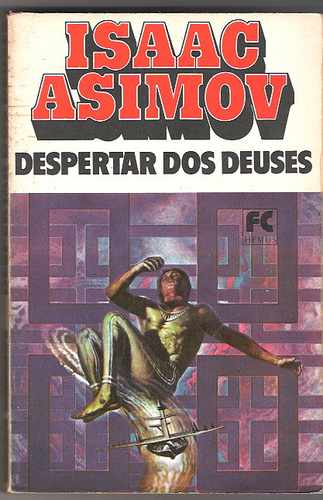
\includegraphics[width=\textwidth]{despertar_deuses_capa}
  \end{figure}
  
  \newpage
  %Asimov Sentado
  \begin{figure}[h]
    \centering
    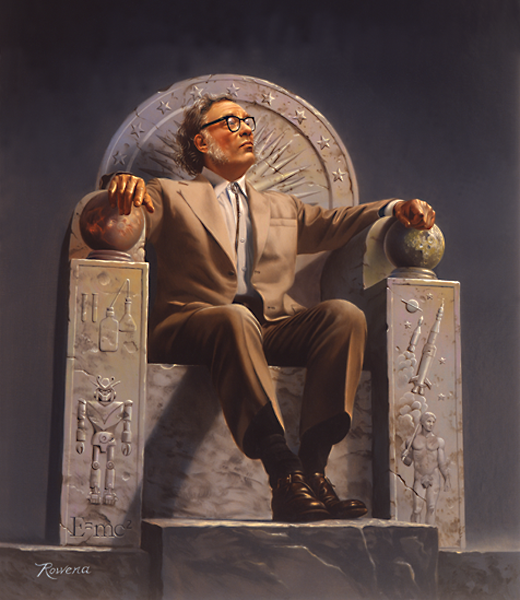
\includegraphics[width=\textwidth]{asimov_sentado}
    \caption{Isaac Asimov}
  \end{figure}

  
  \chapter{Introdução}

    \section{Apresentação da disciplina e do livro}
      
      A disciplina Engenharia e Sociedade aborda o conteúdo ético
      e moral que nós, como graduandos em engenharia, devemos
      exercitar ao seguirmos nossa profissão. Servindo assim como ponte
      entre a capacitação técnica e a sensibilidade social.
      
      Utilizaremos o livro de Isaac Asimov, O Despertar dos Deuses,
      que possui como sinopse:
      
      \begin{quotation}
	Que peripécias viverá a humanidade no futuro? Num mundo que sobreviveu a
	tremenda crise ecológica e que tem fome de energia? Quais os problemas que
	enfrentará? Do contato da Terra com um desconhecido Universo paralelo
	surgem terríveis enigmas imprevistos. Como evitar a catástrofe, que virá com a
	subversão das leis da natureza, se, contra a estupidez humana, os próprios
	deuses disputam em vão?
	
	Da Terra, à beira da tragédia, somos levados por Isaac Asimov ao estranho e
	misterioso Universo paralelo, onde seres dotados de inteligência se conduzem
	de acordo com padrão de vida completamente estranho ao nosso. E dali somos
	transferidos ao mundo Selenita, com a sua colônia humana já estabelecida e já
	desenvolvendo novas formas de convivência social. A essas situações
	fascinantes se acrescenta a emoção das paixões conflitantes de personagens
	inesquecíveis desenhados com invulgar maestria literária. Protagonistas de
	episódios cuja sucessão alucinante não esconde uma meditação profunda, em
	verdade projetada no futuro a partir da experiência crucial de nossa era.
      \end{quotation}

    \section{Objetivos do trabalho}
    
      Nesse projeto utilizamos a leitura do livro de Isaac Asimov, O
      Despertar dos Deuses, para fazermos uma analogia a respeito de
      como a humanidade em geral reagiria face a descoberta de uma
      solução energética que talvez pusesse a Terra ou até o universo em
      risco. Além do outro lado, qual grau de responsabilidade teria uma
      sociedade que solucionaria o problema da morte iminente de seu
      “Sol” colocando, conscientemente, em risco de extinção um outro
      universo. Trançamos um paralelo com a nossa formação e com o
      que significa ser um engenheiro. Além disso, a leitura do livro
      estimulou uma análise conceitual sobre personalidade do ponto de
      vista de que a psique possui três partes, e este conceito foi
      explicado ao fim.
      
    \section{Breve biografia de Isaac Asimov}
    
      Isaac Asimov nasceu em Petrovichi shtetl ou Oblast de
      Smolensk, República Soviética Russa (hoje província de Mahilou,
      Bielorrússia), filho de Anna Rachel Berman Asimov e Judah Asimov,
      um moleiro de uma família de Judeus. Em virtude das diferenças
      entre o calendário hebraico e o calendário juliano (à época ainda em
      uso na região pela Igreja Ortodoxa), bem como pela falta de
      registros, sua data de nascimento não pode ser precisada, situando-
      se entre 4 de outubro de 1919 e 2 de janeiro de 1920, sendo esta
      última considerada como a correta por Asimov, que semprecelebrou seu 
      aniversário a 2 de janeiro. A família deriva seu nome de
      {\cyr ozimiye} (ozimiye), uma palavra da língua russa que significa um
      cereal de inverno que o seu bisavô negociava, ao qual o sufixo
      paterno foi adicionado. Sua família emigrou para os Estados Unidos
      quando ele tinha só três anos de idade. Como seus pais falavam
      sempre iídiche e inglês com ele, ele nunca aprendeu russo. Enquanto
      crescia em Brooklyn, Nova Iorque, Asimov aprendeu a ler, por si
      próprio, quando tinha cinco anos e permaneceu fluente em iídiche,
      bem como em inglês. Seus pais tinham uma loja de doces, e toda a
      gente da família tinha de lá trabalhar. Revistas baratas de papel de
      polpa, chamadas pulp sobre ficção científica eram vendidas em lojas,
      e ele começou a lê-las. Por volta dos onze anos, começou a escrever
      histórias próprias e, por volta dos dezenove anos, tendo-se tornado
      fã de ficção científica, começou a vender suas histórias a revistas.
      John W. Campbell, o editor de Astounding Science Fiction,, para
      quem ele vendeu suas primeiras histórias, foi uma forte influência
      formativa e tornou-se um amigo.
      
      Asimov foi aluno das New York City Public Schools (escolas
      públicas de Nova Iorque), inclusive a Boys' High School, de Brooklyn.
      A partir daí, ele foi para a Universidade de Columbia, onde se
      graduou em 1939, depois tirando um Ph.D. em bioquímica, em 1948.
      Entretanto, passou três anos, durante a Segunda Guerra Mundial, a
      trabalhar como civil na Naval Air Experimental Station, do porto da
      Marinha em Filadélfia. Quando a guerra acabou, ele foi destacado
      para o Exército Americano, tendo só servido nove meses antes de
      ser honrosamente reformado. Durante sua breve carreira militar, ele
      ascendeu ao posto de cabo, baseado na sua habilidade para escreverà máquina, 
      e escapou por pouco de participar nos testes da bomba
      atómica em 1946 no atol de Bikini.
      
      Depois de completar seu doutorado, Asimov entrou na
      faculdade de Medicina da Universidade de Boston, com a qual
      permaneceu associado a partir daí. Depois de 1958, isto foi sem
      ensinar, já que se virou para a escrita em tempo integral (suas
      receitas da escrita já excediam as do salário acadêmico). Pertencer
      ao quadro permanente significou que ele manteve o título de
      professor associado e, em 1979, a universidade honrou sua escrita
      promovendo-o a professor catedrático de bioquímica. Os arquivos
      pessoais de Asimov, a partir de 1965, estão arquivados na Mugar
      Memorial Library da universidade, doados por ele a pedido do
      curador, Howard Gottlieb. A colecção preenche 464 caixas em 71
      metros de prateleira.
      
      Asimov casou-se com Gertrude Blugerman (Canadá, 1917 —
      Boston, 1990), em 26 de julho de 1942. Tiveram duas crianças, David
      (n. 1951) e Robyn Joan (n. 1955). Depois da separação, em 1970, ele
      e Gertrude divorciaram-se em 1973, e Asimov casou-se com Janet O.
      Jeppson mais tarde, no mesmo ano.
      
      Asimov era um claustrofilo; gostava de espaços pequenos
      fechados. No primeiro volume da sua autobiografia, ele conta um
      desejo infantil de possuir uma banca de jornais numa estação de
      metrô de Nova Iorque, dentro da qual ele se fecharia e escutaria o
      ruído dos carros enquanto lia.
      
      Asimov tinha medo de voar, só o tendo feito duas vezes na vida
      inteira (uma vez, durante seu trabalho na Naval Air Experimental
      Station, e outra, na volta para casa da base militar de Oahu, em1946). 
      Raramente viajava grandes distâncias, em parte por causa de
      sua aversão a voar, adicionada às dificuldades logísticas de viajar
      longas distâncias. Esta fobia influenciou várias das suas obras de
      ficção, como as histórias de mistério de Wendell Urth e as novelas
      sobre robôs de Elijah Baley. Nos seus últimos anos, ele gostava de
      viajar em navios de cruzeiro e, em várias ocasiões, ele fez parte do
      "entretenimento" no cruzeiro, dando palestras baseadas em ciência,
      em navios, como os RMS Queen Elizabeth 2. Asimov sabia entreter
      muitíssimo bem, era prolífico e procurado como discursador. Seu
      sentido de tempo era fantástico; ele nunca olhava para um relógio,
      mas invariavelmente falava precisamente o tempo combinado.
      
      Asimov era um participante habitual em convenções de ficção
      científica, onde ficava amável e disponível para conversa. Ele
      respondia pacientemente a dezenas de milhares de perguntas e
      outro tipo de correio com postais, e gostava de dar autógrafos.
      Embora gostasse de mostrar seu talento, raramente parecia levar-se
      a si próprio demasiadamente a sério.
      
      Ele era de altura mediana, forte, com bigode e um óbvio
      sotaque de judeus do Brooklyn. Seu físico era bastante limitado. Ele
      nunca aprendeu a nadar ou andar de bicicleta; no entanto, aprendeu
      a conduzir um carro, depois de se mudar para Boston. No seu livro
      de humor, Asimov Laughs Again, ele descreve a condução em Boston
      como "anarquia sobre rodas".
      
      Ele demonstrou seu amor por conduzir, em seu conto de ficção
      científica, Sally, sobre carros-robôs. Um leitor atento reparará que
      ele faz uma descrição detalhada de um dos carros a que chama
      'Giuseppe', de Milão - o que significa que Giuseppe era um AlfaRomeo. 
      Asimov não especificou nenhum outro tipo de veículo em
      nenhuma das suas histórias, o que levou muitos fãs a considerarem
      que ele foi contratado por aquela marca de automóvel.
      
      Os interesses variados de Asimov incluíram, nos seus anos
      tardios, sua participação em organizações devotadas à opereta de
      Gilbert and Sullivan e em The Wolfe Pack, um grupo de seguidores
      dos mistérios de Nero Wolfe, escritos por Rex Stout. Ele era um
      membro proeminente da Baker Street Irregulars, a mais importante
      sociedade sobre Sherlock Holmes. De 1985 até sua morte em 1992,
      ele foi presidente da American Humanist Association; seu sucessor
      foi o amigo e congênere escritor, Kurt Vonnegut. Ele também era um
      amigo próximo do criador de Star Trek, Gene Roddenberry, e foram-
      lhe dados créditos em Star Trek: The Motion Picture, pelos conselhos
      que deu durante a produção.
      
      Asimov morreu em 6 de abril de 1992 em Nova Iorque. Foi
      cremado e suas cinzas foram espalhadas. Ele deixou sua segunda
      mulher, Janet, e as crianças do primeiro casamento. Dez anos depois
      da sua morte, a edição da autobiografia de Asimov, It's Been a Good
      Life, revelou que sua morte foi causada por AIDS; ele
      contraiu o vírus HIV através de uma transfusão de sangue recebida
      durante a operação de bypass em Dezembro de 1983. A causa
      específica da morte foi falha cardíaca e renal, como complicações da
      infecção com o vírus da AIDS.
      
      Janet Asimov escreveu no epílogo de It's Been a Good Life que
      Asimov o teria querido tornar público, mas seus médicos
      convenceram-no a permanecer em silêncio, avisando que o
      preconceito anti-AIDS estender-se-ia a seus familiares. A família de
      Asimov considerou divulgar sua doença antes de ele morrer, mas a
      controvérsia que ocorreu, quando Arthur Ashe divulgou que ele
      tinha AIDS, convenceu-os do contrário. Dez anos mais tarde, depois
      da morte dos médicos de Asimov, Janet e Robyn concordaram que a
      situação em relação à AIDS podia ser levada a público.
      
  \chapter{Resumo}

    \section{Contra a estupidez...}
    
      A história começa com um estranho acontecimento, quando
      cientistas descobrem que uma amostra de Tungstênio-186 foi trocada
      por outra de Plutônio-186. Acontece que o Plutônio-186 não é estável e
      nem mesmo possível, segundo as leis da física conhecidas, e por isso, em
      pouco tempo o elemento perde a sua estabilidade e começa a liberar
      radiação. O radioquímico Frederick Hallam cria a teoria de que este
      elemento teria vindo de um outro universo, onde as leis da física
      pudessem aceitar a existência do mesmo. O elemento ao chegar ao
      nosso universo seria capaz de se manter estável, por trazer parte de seu
      verdadeiro universo, mas com o tempo, o nosso universo conseguia
      fazer valer suas leis sobre ele e o Plutônio-186 se desestabilizava.
      
      Através das experiências de trocas dos elementos, os cientistas
      recebem placas enviadas por seres deste ”outro universo” (Para-
      Universo), onde eles descreviam como criar uma máquina que faria a
      troca de elementos dos dois lados, recebendo a Terra o Plutônio-186, e
      enviando para eles o Tungstênio-186 (assim como Plutônio-186 em
      nosso mundo, o Tungstênio-186 seria instável e radioativo no Para-
      Universo). Esta máquina (chamada de ”Bomba Eletrônica”) seria capaz
      assim de criar energia radioativa cíclica e infinita, para os dois lados.
      
      O cientista Benjamin Allan Denison chega à conclusão de que tal
      bomba traria a ruína ao nosso universo. Com a troca constante de ”leis”
      entre os dois universos, suas regras se misturariam e tudo que faz o
      nosso universo funcionar se desestabilizaria aos poucos. Isto foi previsto
      pelo Dr. Hallam, mas num prazo de bilhões de anos. De acordo com
      Denison, isso podia acontecer em menos de cem anos.
      
      Investigando os fatos e indivíduos envolvidos em torno da criação da
      Bomba Eletrônica, o jovem Dr. Peter Lamont chega a conclusão de que
      esta poderia significar a aniquilação do Universo. Ele passa a investigar
      a tradução das placas enviadas pelos seres do Para-Universo com a ajuda
      de um perito linguístico, Dr. Myron Bronowski. A situação complica-se
      quando começam a surgir placas com mensagens de que a Bomba seria
      perigosa, ao mesmo tempo em que os esforços de Lamont em provar
      sua teoria da possível destruição não são reconhecidos.

    \section{...Os próprios deuses...}

      A segunda parte do livro descreve a vida no para-Universo. Somos apresentados
      dois tipos de criaturas, os Suaves e os Durões. Os Suaves são seres sem forma definida,
      como se fosse uma nuvem de gás, podendo alterar sua forma a seu bel-prazer e até penetrar em outros objetos. 
      Os Suaves são dividos em três gêneros, os Racionais (ou Esquerdistas), os Parentais (ou Direitistas), 
      e as Emocionais (ou Intermediárias). Cada gênero possui comportamento e responsabilidades
      bem definidas, e esses seres se organizam em tríades, com um elemento de cada gênero. A história
      é contada do ponto de vista de uma tríade, composta por um Racional chamado Odeen, um Parental chamado Tritt,
      e uma Emocional chamada Dua.
      
      Os Racionais são seres com extrema capacidade de aprendizado e racíocinio. São vistos como os líderes das tríades,
      e são os únicos a manter contato constante com os Durões, que atuam como mentores para os Racionais. Na reprodução 
      os Racionais são responsáveis por fornecer a semente para gerar um novo indivíduo. O corpo dos Racionais possui curvas
      suaves, mas mantendo uma forma definida. Os Racionais passam o dia estudando e aprendendo com os Durões.
      
      Os Parentais são responsáveis pela gestação dos filhos. Para um Parental a única coisa que importa na vida é
      gerar seus três filhos, que sempre ocorre na mesma ordem: primeiro o filho Racional, depois o filho Parental e por último
      a filha Emocional. Os Parentais não conseguem pensar logicamente como os Racionais, mas em contrapartida possuem uma
      forte intuição, a qual guia suas ações. Dos três gêneros, os Parentais são os mais corpulentos, com formas quase rígidas.
      Os Parentais dedicam seu dia inteiro para cuidar dos filhos.
      
      As Emocionais possuem uma grande sensibilidade, em determinadas situações podendo até sentir o ambiente a sua volta, como
      saber a localização de outros seres mesmo sem enxergá-los ou ouví-los. Enquanto os outros gêneros também apresentam essa
      capacidade em determinadas situações, as Emocionais possuem essa habilidade mais desenvolvida. Durante a reprodução,
      a Emocional age como intermediadora, ela é reponsável por facilitar o processo e fornecer a energia necessária para que uma
      nova vida seja formada. Dos três gêneros, a Emocional possui o corpo menos denso de todos, e por isso é capaz de modificar sua
      forma com maior facilidade. A diferença de densidade também interfere no comportamento das Emocionais: enquanto os Parentais e
      Racionais precisam de poucos minutos no Sol para se alimentar, as Emocionais passam horas na superficie para conseguir comer
      e acumular energia suficiente para gerar uma nova vida.
      
      Os Durôes são seres parecidos com as formas de vida que conhecemos. O livro explora pouco os Durões, uma vez que eles procuram
      manter distância da vida cotidiana dos Suaves, com excessão dos Racionais. Eles possuem corpos sólidos, diferente dos Suaves.
      Os Durões são os líderes do planeta onde vivem com os Suaves, e são responsáveis por tentar solucionar um problema que oferece
      um grande perigo para ambos: a estrela que fornece energia para o planeta está esfriando.
      
      O Sol possui uma enorme importância para os seres do para-Universo, pois é de sua energia que os Suaves se alimentam. Com o esfriamento
      do Sol, os Suaves se alimentam cada vez menos (principalmente as Emocionais, que necessitam de mais energia que os outros dois gêneros) e
      com isso a população de Suaves e Durões está declinando. Por esse motivo, os Durões desenvolvem a Bomba Eletrônica, um meio de trocar energia
      com o Universo humano a fim de alimentar os Suaves com energia "artificial". Entretanto, a Bomba Eletrônica não troca apenas energia, uma de suas
      funções é trocar as leis físicas básicas dos dois Universos, o que causaria a explosão do Sol do nosso Universo e um acumulo de energia no Sistema
      Solar, de onde os Durões poderam captar energia ilimitadamente.
      
      Tanto os Durões quanto os Suaves vivem em cavernas no subsolo. A superficie do planeta só é visitado pelos Suaves, que vão se alimentar ao Sol. Os Parentais
      e Racionais ficam apenas poucos minutos, pois são mais densos e absorvem a energia mais rápido. Já as Emocionais precisam ficar horas ao Sol para conseguir
      se alimentar, além delas serem menos densas, as Emocionais precisam acumular mais energia para gerar uma nova vida durante o derretimento.
      
      O derretimento é o equivalente ao sexo para os Suaves. Durante o derretimento, a Emocional se rarefaz e se espalha pelo ambiente, permeando ambos o Racional e o Parental.
      Os outros dois também se esticam, mas não possuem a mesma capacidade da Emocional. O Parental então cria um apêndice comprido que penetra a pele do Racional, para transportar
      a semente do Racional para o Parental. Após o climax a tríade perde a consciência por um tempo, as vezes até por alguns dias. A tríade não recobra nenhuma lembrança desse período
      inconsciente, somente alguns lampêjos, da mesma forma que acontece com um sonho. Após um derretimento, o Parental pode começar a gerar um filho. 
      Como mencionado antes, isso depende da Emocional, que deve fornecer energia suficiente durante o derretimento para formar a nova vida. 
      
      Gerados os três filhos, chega o momento da tríade seguir adiante. O Racional é responsável por determinar quando é o momento correto de seguir adiante, que é
      o momento em que a tríade deixará de existir. O livro deixa subentendido que seguir adiante significa a morte, que é como os Suaves entendem. Na verdade, seguir adiante significa 
      que a tríade deixará de ser Suave e se junta para formar um Durão. Os Suaves e Durões não são duas espécies diferentes, apenas dois estágios de maturidade de um único ser. 
      O período de insconsciência após o derretimento é uma união temporária dos Suaves em um Durão. O momento de seguir adiante é quando o Racional da tríade atinge maturidade suficiente
      para descobrir a verdade sobre seguir adiante. É importante que ele perceba por si próprio, sem influência de outros Racionais ou Durões, para não prejudicar seu desenvolvimento. 
      Quando o Racional chega a essa conclusão, ele conta para o Parental e a Emocional, que então vão derreter uma última vez para formar um Durão permanentemente.

      \subsection{Capitulo 1a}
      
	O capitulo 1a começa falando sobre Dua, e sua relação com Odeen e Tritt. Dua era diferente dos outros Emocionais, ela gostava de vagar sozinha, e isso incomodava Tritt. Odeen, por sua vez,
	tentava interceder com Tritt, a fim de acalmá-lo, mas ultimamente isso não era tão mais necessário, pois Tritt estava sempre cuidando das crianças. Dua relata que não se importa com Tritt,
	mas Odeen causava uma atração sobre ela.
	
	Dua relembra sua infância, desde muito nova sempre foi tratada como diferente pelos demais Emocionais. Ela gosta de sair para a superfície ao entardecer, o que era incomum pois nessa hora o Sol
	está fraco. Para Dua se alimentar nesse horário remete a liberdade.
	
	Ela relembra então de seu Parental, que vinha atrás dela quando ela fugia, com medo de Dua se ferir. Em um dia específico, Dua estava se alimentando ao por do sol quando seu Parental veio lhe dizer
	que ele iria seguir em frente. Ele pede que Dua ouça seus irmãos mais velhos depois que ele se for. Dua protesta porque ressente o afastamento de seus irmãos que, mais velhos, tinham outras preocupações.
	Ela também ressente as outras Emocionais, que só pensam em se alimentar, formar tríades e fofocar. Dua questiona porque seu Parental deve seguir adiante, e ele responde que deve seguir a hora que o
	seu Racional escolher. Dua chora enquanto seu pai vai embora para sempre.
	
      \subsection{Capitulo 1b}
	
	Odeen reflete sobre Dua. Ele consegue sentí-la se aproximando, voltando da superfície. As tríades possuem uma interconsciência, cada individuo pode sentir os outros se ele se concentrar para isso.
	Odeen pensa sobre seguir adiante. 
	
	%TODO: Terminar seção 1b
	
      \subsection{Capitulo 1c}
      
	Tritt indaga Odeen sobre o paradeiro de Dua. Ele se incomoda com a indiferença dela com relação a tríade. Tritt pressiona Odeen sobre o terceiro filho e a pouca alimentação de Dua. Tritt acredita
	que Odeen se preocupa com coisas fúteis, como átomos e energia, e não com a tríade, que no seu ver é o que realmente importa. Tritt acha que o motivoda redução do número de Suaves se deve as pessoas não
	se importando mais com as tríades.
	
	Tritt se recorda de como obteve Dua. Em um momento impetuoso, ele abordou um Durão, Losten, sobre a necessidade de um Emocional para completar a tríade. Isso envergonhou Odeen, que estava presente e 
	achou que Tritt estava incomodando ou até insultando Losten. Ele diz que Tritt deve ser paciente, e que os Durões estão decidindo quem será a Emocional escolhida para sua tríade.
	
	Um tempo depois, Losten trouxe Dua. Tritt ficou apaixonado, e instantaneamente percebeu que nenhuma outra Emocional teria servido para sua tríade. Instintivamente, os três começaram a derreter.
	Dua afinou. Tritt imergiu na névoa que era Dua, e também afinou, sem a dificuldade de antes. Odeen fez o mesmo. Odeen e Tritt deslizaram para dentro um do outro, atingiram um orgasmo, e os três perderam
	a consciência.
	
	A tríade derreteu por dias. Após acordarem, Dua disse que precisava sair, e que depois fariam isso de novo. Dua sempre faz isso depois de derreter, o que aborrecia Tritt pois esse comportamente não é
	normal. Odeen e Tritt discutem sobre isso, e Tritt se cala, sem conseguir expressar tudo o que pensa.
    
    \section{...Disputam em vão?}
    
      O desfecho do livro é protagonizado pelo Dr. Denison, o ex-colega de
      Frederick Hallam, ridicularizado por ele na época primeira da descoberta
      da amostra de Plutônio-186. Denison viaja até a Lua, procurando na
      colônia selenita um recomeço para sua carreira que fora destruída na
      Terra por Hallam. Lá conhece Selene, uma selenita que serve de guia a
      ele no diferente ambiente lunar. Logo, Denison vê-se novamente
      envolvido com os problemas da Bomba Eletrônica e se torna a peça
      chave para explicar as teorias que comprovam seu perigo e por elaborar
      uma possível solução para todo o problema.
        
    \section{Dilema “Energia infinita e barata”}

      O livro se baseia na conjuntura que a Bomba Eletrônica produziria energia sem custos, e com isso, a humanidade atingiria um estado quase utópico. 
      Entretanto, essa utopia só acontece em um certo aspecto da sociedade, outros problemas perduram, estes que levam quase a destruição da Terra.

      Podemos traçar um paralelo com a humanidade hoje. 
      Embora não tenhamos uma fonte energética com as mesmas qualidades que a Bomba Eletrônica, o petróleo é semelhante à Bomba no seu custo, 
      além de também apresentar uma consequência ambiental negativa.

      Assim como descrito no livro, a humanidade parece não ser capaz de extinguir o uso do petróleo, 
      apesar dos problemas ambientais causados pela queima de combustíveis fósseis. 
      Essa é outra semelhança do livro com a realidade, pois há pessoas que negam os efeitos negativos causados pelo petróleo, 
      assim como as ideias de Lamont foram refutadas. Poucos são os governantes dispostos a colocar o crescimento de seu país 
      em segundo plano, substituindo fontes baratas de energia por outras de maior custo, mas de menor impacto ambiental.

      Da mesma forma, poucas pessoas estão dispostas a abandonar o uso de derivados de petróleo em prol de outras fontes de 
      energia alternativas, seja por motivos econômicos ou pessoais. No livro o autor deixa bem claro, o bem-estar e os interesses 
      do indivíduo estão acima do coletivo. Isso ocorre pois o ser humano tem um desejo inerente de querer avançar, melhorar, evoluir. 
      Esse desejo ao mesmo tempo que motiva o Homem a realizar grandes feitos, pode cegá-lo, não permitindo nenhuma forma de retrocesso 
      ou estagnação, não importando as consequências desse crescimento desenfreado.

      A tirinha a seguir exemplifica este comportamento. Uma vez atingido um patamar de desenvolvimento, não é aceito retornar aos padrões anteriores, 
      mesmo que para manter o status quo sejam necessários sacrifícios, no caso da tirinha, da vida do Super-Homem.
      
      %Quadrinho superman
      \begin{figure}[h]
	\centering
	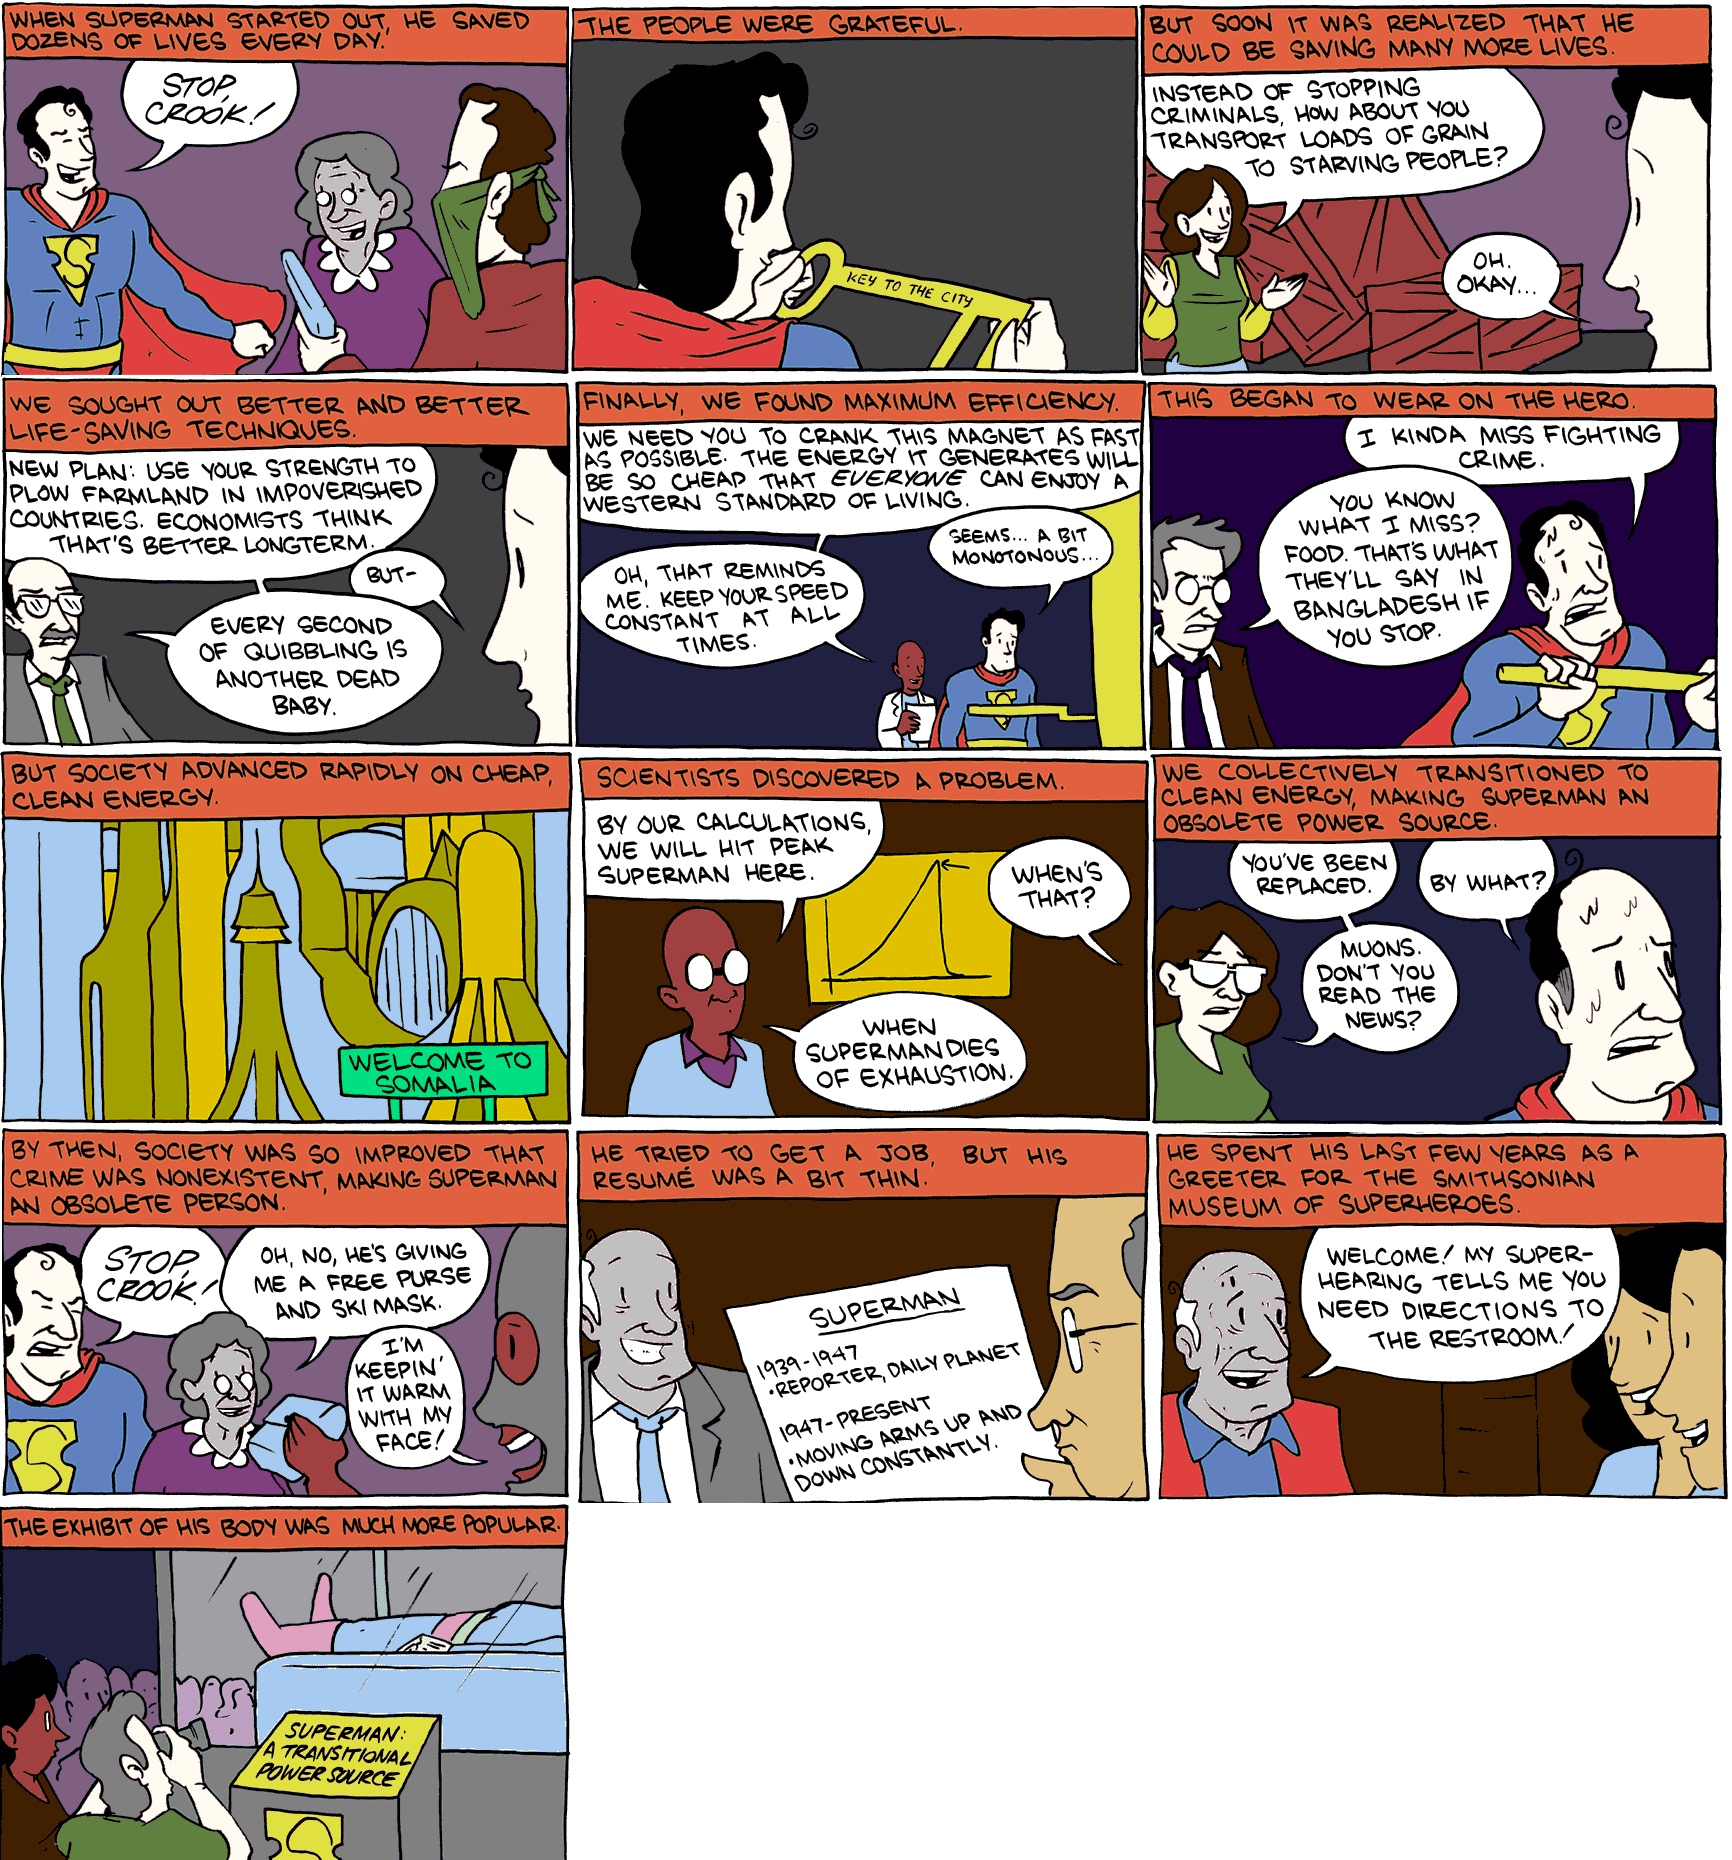
\includegraphics[width=\textwidth]{comic_superman}
	\caption{Super-homem como fonte de energia}
      \end{figure}
        
  \chapter{O Despertar dos Deuses e a Engenharia Contemporânea}

      Engenharia é “a capacidade de aplicar os conhecimentos científicos
      de forma prática a fim de produzir novas utilidades. Para obter tais
      resultados, o engenheiro estuda o problema, planeja uma solução,
      verifica a viabilidade econômica e por fim coordena o desenvolvimento
      ou produção”. Porém, hoje a utilidade também tem que ser sustentável.

  \chapter{O conceito das três partes}

    A ideia passada pelo texto de uma espécie dividida em três partes
    complementares, que precisam entrar em harmonia para completar o
    ser, incentivou uma análise da mente humana de forma similar. Esse
    conceito foi trabalhado por meio de comparações com o
    comportamento de pessoas reais de forma a maturar em um modelo no
    mínimo interessante que abre caminho para discussões filosóficas,
    sobre a necessidade da diversidade e os motivos de dissidências entre
    diferentes linhas de pensamento, por outra perspectiva. A ideia é
    descrita a seguir em tom de fenômeno físico observado mas não almeja
    ser tratado como um modelo da complexidade da mente humana. A
    termodinâmica é uma valida representação dos valores médios
    populacionais da mecânica estatística e a psicologia tentar fazer este
    papel em relação à neurologia. Da mesma, forma o modelo de três
    partes pode, talvez, representar bem as médias, sem qualquer
    conhecimento da complexidade humana.
    
    Dentro deste modelo, a mente fica dividida em três partes, chamadas
    de partes conservadora, dinâmica e racional. Um indivíduo pode nascer
    com uma destas partes melhor desenvolvida que as outras, e isso defineo seu modo de pensar, mas pode, e deve, desenvolver as três partes
    durante a sua vida. O desbalanceamento das três partes em um
    indivíduo, A, causa a incapacidade deste indivíduo compreender os
    pensamentos de outro indivíduo, B, que partem de uma das partes não
    desenvolvidas por A. Além da clara dificuldade de trabalhar em conjunto
    e respeitar outros pontos de vista, por considerar errados, um indivíduo
    A com uma das três partes mais desenvolvida do que as outras pode
    passar a não utilizar suas partes menos desenvolvidas por completo.

    \section{A analogia}
    
      Na segunda parte do livro “O Despertar dos Deuses”, “...os próprios
      deuses...”, o paternal, o emocional e o racional, de início tão
      desconectados e centrados em suas capacidades e modus operandi
      naturais, passam a se compreender cada vez mais, e, como
      consequência disso, não somente passam a atuar melhor em conjunto
      como também desenvolvem capacidades adicionais advindas do meio
      termo entre suas personalidades. Por fim estes entram em equilíbrio se
      tornando um só ser de capacidade maior do que a soma de suas
      capacidades individuais. Deste ponto principal da segunda parte do livro
      e da descrição das divergências de formas de pensar e agir dos três
      gêneros de “suaves”, o conceito do ser humano como uma composição
      de três “suaves” em desequilíbrio aparentemente explica as
      personalidades extremas e personalidades intermediarias encontradas
      pelo mundo, além de explicar suas convergências e divergências.
      
    \section{O conservador}
    
      O lado conservador está associado aos princípios básicos de
      sobrevivência de nosso ego. Diferente de racionalidade, um conjunto
      básico de regras imutáveis na forma de um “look-up table” tornam o
      sujeito majoritariamente conservador rápido e produtivo. Não existe
      muita margem para discussões ou mudanças, o conservador tem suas
      verdades bem definidas e uma memória longa, pouco “fator de
      esquecimento”, reforçando a primeira impressão sobre um assunto ou
      pessoa.
      
      Enquanto suas verdades não forem abaladas, o majoritariamente
      conservador é o mais confiável, por ser o mais previsível, e o mais
      produtivo, por não desviar de suas metas e conduta moral. O
      conservador não entra em discussões filosóficas sobre o sentido de sua
      vida, ele segue alguma crença divina ou senso moralista de justiça que é
      inabalável pela racionalidade alheia. Quando, de fato, o conservador
      perde sua crença, por se apoiar totalmente nela, ele fica completamente
      perdido.
      
      A associação desse comportamento com o funcionamento baseado
      em princípios básicos de sobrevivência é simples. Nossos instintos
      básicos são de cautela. Com memórias longas e enfáticas nas primeiras
      experiências, um animal não se aproxima de possíveis perigos e se
      preserva, mesmo quando desnecessariamente, mesmo quando não há
      um perigo real. “Better safe than sorrow”. Já o funcionamento por base
      em regras básicas e não por racionalidade é facilmente explicado pelo
      fato de que, na natureza, as vezes qualquer reação imediata vale mais
      do que uma reação pensada segundos depois. Correr para longe de um
      barulho repentino pode salvar a sua vida, enquanto tentar raciocinar se
      o barulho merece atenção ou não pode causar sua morte. Neste caso,
      correr a toa vale mais do que pensar se vale a pena correr. É claro que,
      da mesma forma que faço aqui, isto pode ser raciocinado previamente,porém, em uma situação repentina, dependeria do tipo da pessoa
      conseguir seguir o “script” ou tentar compreender a situação. O “medo”
      do desconhecido pode ser a reação certa a se ter, enquanto o indivíduo
      majoritariamente racional perderia tempo raciocinando sua reação no
      momento em que já deveria estar tomando alguma ação.
      
      Deve ser enfatizado que a característica principal do conservador é a
      auto preservação. Mudanças não são sempre evitadas apesar de sempre
      haver reclamação. Quando uma mudança acontece repentinamente, o
      reflexo do conservador é querer voltar para a situação anterior mesmo
      que isto seja impossível, pois nela ele sabe que sobrevive. Qualquer
      mudança subsequente que aproxime a situação atual à antiga será
      aceita e, depois, criticada. “Não está tão bom quanto antes”
      
      Fica aparente uma dicotomia entre o racional e o conservador neste
      quesito mas também existem uma dicotomias aparentes entre o
      dinâmico e o racional e entre o dinâmico e o conservador, mostrando o
      quão complementares estas ideias são. São estas aparentes dicotomias
      que criam os conflitos internos no indivíduo que tem dois “suaves”
      relativamente equilibrados mas a ausência do terceiro.
      
      O lado conservador se apresenta como um resquício evolutivo mas
      isso não justificaria uma maioria da população mundial
      majoritariamente conservadora, que de fato é o que pode ser
      constatado pensando melhor no assunto. Seria o mesmo que dizer que
      a população mundial está, em média, em sua infantilidade evolutiva.
      Esta situação pode ser melhor elaborada com a analogia à genética.
      
      \subsection{Analogia Genética}
      
	Pensando em seres mais primitivos, como bactérias unicelulares,
	vemos que seu código genético possui poucos mecanismos depreservação. Devido à isso, durante a replicação, muitas mutações
	acontecem causando grande diversidade. Para seres simples, isto pode
	ser visto majoritariamente como vantagem porém, para seres
	complexos e pluricelulares, isto pode fazer com que blocos funcionais,
	como o código para a mão ou o fígado, sejam modificados para algo não
	funcional. Para que isso não aconteça, foi necessário o desenvolvimento
	de formas mais conservadoras de replicação genica, com verificação e
	correção do código após replicação e modificações feitas por troca de
	blocos funcionais inteiros entre diferentes alelos, “crossing-over”, de
	forma a manter a evolução, porem de forma menos dinâmica
	preservando blocos funcionais.
	
	Da mesma forma, uma população que não fosse majoritariamente
	conservadora implicaria numa grande massa de pensamento
	divergente, causando revoluções constantes, não necessariamente para
	melhor, reduzindo a produtividade total. Se todos estão preocupados
	em criar novas ferramentas para o plantio, ninguém está plantando
	nada e todos vão morrer de fome. Se muitos gastam o dia discutindo
	sobre quais religiões estão erradas, os conservadores que tem lastro
	nessas religiões perdem produtividade por influência da inserção de
	dúvidas, enquanto os que discutem em si não produzem nada.
	
    \section{O dinâmico}
      
      Ao contrário do conservador, o dinâmico não utiliza nenhum tipo de
      lastro e não se apoia em memória. Está constantemente buscando
      modificações e sempre insatisfeito. Este lado é baseado em nossa
      necessidade de evoluir. Assim como em algoritmos genéticos, na
      verdade exatamente como, todos os humanos dão saltos randômicos de
      opinião e forma de pensar. Estas são questionadas e pontuados, claroque essa pontuação só será eficiente com o desenvolvimento racional,
      e novos passos são dados de forma a encontrar ótimos locais. O princípio
      do “suave” dinâmico é o que impede que o ser convirja em máximos
      locais. É a “mutação” no algoritmo genético que impede que se convirja
      em um máximo local, possibilitando que se alcance o máximo global.
      Esse papel aleatório deve ser o princípio da criatividade. Fica claro de
      antemão que a calibração das três partes em uma população deve
      funcionar analogamente a calibração de um algoritmo genético.
      
      O majoritariamente dinâmico acaba sendo um indivíduo
      improdutivo, que passa seus dias filosofando sobre tudo, invés de
      produzindo algo, mas sem a racionalidade necessária para chegar a
      conclusões. Instável e de difícil convivência, normalmente não é
      respeitado pelos majoritariamente conservadores por serem inúteis
      nem pelos majoritariamente racionais por serem irracionais.
      
      Vendo que o cérebro humano processa mais informação do que o
      ego tem consciência de, podemos conjecturar a possibilidade de utilizar
      esta informação. Isto poderia justificar a sensação de estar sendo
      observado de uma direção fora do seu campo de visão. O
      processamento paralelo de toda a informação de todos os sensores do
      corpo humano pode acionar alarmes para nosso ego sem que as
      informações necessárias para chegar nestas conclusões sejam todas
      entregues. O dinâmico desenvolve seu lado intuitivo e talvez se torne
      mais receptivo aos “alarmes” do cérebro. Isto possibilitaria tomar uma
      decisão correta sem ter a capacidade de compreender a situação por
      completo. Como o teorema de Gödel mostra que um sistema só
      consegue compreender outro sistema mais simples que ele mesmo, e
      existem muitos sistemas mais complexos que o sistema racional quecompõe o ego, o “suave” dinâmico contornaria este problema
      recebendo informações do sistema neural completo, além do ego.
      
      O processamento linear e sequencial da racionalidade matemática
      possui limites pelo seu sistema inerente, o ego humano, enquanto o
      sistema neural completo, com processamento paralelo, ultrapassa a
      linha racional de pensamento. A compreensão sem compreender é
      marca deste tipo dinâmico, que “sente” a resposta ao invés de raciocina-
      la. Apesar de parecer uma característica artística mais do que científica,
      parece ser o diferencial de homens como Einstein ou Newton, que
      conjecturavam ideias corretas sobre o universo mesmo que contra
      intuitivas ao racionalismo aplicado ao conhecimento da época. De fato,
      o estado-da-arte apresenta uma característica de “feeling” que pouco
      pode ser descrita como resultado de pensamento matemático linear
      racional.
      
      Mesmo tentando explicar este “sentimento” em cima das
      informações, o funcionamento do “suave” dinâmico parece exceder a
      simples utilização da habilidade inerente do cérebro de processamento
      paralelo, assim como é difícil de caracterizar a criatividade por algo não
      estocástico. Talvez seja a falta de conservadorismo que possibilite que
      fleches de ideias, que surgem randomicamente em nossas mentes, se
      propaguem o suficiente para se tornar um conceito trabalhado. As vezes
      isso pode gerar ideias descartáveis e erradas mas também pode levar a
      verdades contra intuitivas.
    
    \section{O racional}
      
      Apesar de parecer auto explicativo e absolutamente positivo, o
      racional possui o defeito de ser racional. Devido aos desenvolvimento
      de Gödel, ficou demonstrado que existe um limite para a compreensãodo universo por parte de um integrante deste universo. Somente pode
      ser compreendido algo de complexidade menor que o sistema que tenta
      o compreender. A ideia de que tudo pode ser compreendido e
      racionalizado está errada e um indivíduo que não consegue contornar
      algo incompreensível pode ficar preso em paradoxos. Além disso, no
      mundo prático, não ter reações na forma de “look-up table” não é
      eficiente em muitos casos, como foi discutido sobre o conservador.
      
      Entre um “suave” puro de cada tipo, o racional ainda é o melhor
      opção como líder.
      
    \section{Psicologia Social}
    
      No âmbito da psicologia social, o modelo das três partes pode
      explicar a “foot-in-the-door technique”, onde, ao se pedir cada vez mais,
      aos poucos, pode-se convencer alguém a algo que não seria possível
      pedindo de uma só vez. Como nenhum indivíduo é puramente
      conservador, sempre é possível lhe convencer à algo ligeiramente além
      do seu comum, desde que não saia muito de suas verdades primárias. O
      estado atual desde indivíduo passa a ser o de quem aceita, também, está
      nova condição. Com o seu “look-up table” atualizado, agora, o processo
      pode ser repetido. Um indivíduo puramente conservador não teria
      aceitado nenhuma forma de persuasão para fora de seu modus
      operandi. No entanto, um majoritariamente conservador permitiria esta
      flexibilidade e, ao mesmo tempo, se basearia em comparar suas
      premissas atuais com o que está sendo pedido para decidir aceitar ou
      não. Isto permite a “foot-in-the-door technique”. Com um indivíduo
      majoritariamente racional ou dinâmico o mesmo não acontece, o
      primeiro por só ser persuadido por razão e o segundo por decidir de
      forma aleatória, na média seria meio a meio de sim e nãos, ou porsentimento, o que não seguiria uma cadeia de aceitações baseadas nas
      aceitações anteriores.
      
      Também pode-se explicar casos como o terceiro Reich e o massacre
      de Ruanda pela maioria ser majoritariamente conservadora, como
      citado previamente. Casos em que as pessoas são levados ao extremo
      aos poucos são possíveis, novamente, pelo conservadorismo que
      enfatiza a situação encontrada mais do que a mudança. O racionalismo
      por outro lado, independente da cultura e situação local, discerne o
      construtivo do destrutivo. Para alguns falta a racionalidade para
      compreender as interconexões existentes entre os indivíduos e entre a
      natureza como um todo, fazendo que estes ajam de forma não
      construtiva e egocêntrica, enquanto em outros o sentimento da ação
      coletiva prevalece mesmo sem uma lógica. Em outros casos, o
      sentimento de interconexão faz com que uma ação seja rejeitada por
      parecer egocêntrica quando na verdade é a melhor ação para o coletivo.
      A inercia social que o conservadorismo causa impede mudanças bruscas
      mas não impede mudanças gradativas. Ao mesmo tempo, impede que
      mude-se a direção em que a sociedade se move, mesmo que em direção
      a um abismo. Em situações de crise e falta de lastro, o conservador é
      levado ao extremo e, ao encontrar uma ideia para se lastrear, fica preso
      e molda sua realidade em cima dela. Após observar resultados positivos
      da política externa do terceiro Reich para a Alemanha, o povo assumiu
      o Reich como sua religião.
      
  \chapter{Conclusão}

   Asimov nos convida a refletir sobre o papel da humanidade e o balanço entre energia farta e barata ao custo do desconhecido, 
   contra o status quo. Basicamente é uma viagem ao interior do psique humana, que é expressa metaforicamente pelos para-seres que 
   denotam as diversas facetas do ser humano em seres distintos. 

   Os paralelos com a carreira na área de engenharia são diversas, dentre elas são citadas as responsabilidades inerentes das aplicações 
   de novas tecnologias, metodologias ou qualquer outra dinâmica que afete a humanidade como um todo. Hoje, por exemplo, muito se fala em 
   energia renovável e só a prudência e o incansável questionamento, erros e acertos das carreiras científicas, engenharias inclusas, dirão 
   o quão renováveis e sustentáveis realmente são. 

   Portanto podemos atribuir à carreira na área de engenharia não só o prestígio, mas a responsabilidade que advém do conhecimento para transformar o mundo.
   
\end{document}
